\documentclass{article}
\usepackage{geometry}
\geometry{a4paper, margin=1in}
\usepackage{enumitem}
\usepackage{graphicx}
\usepackage[hidelinks]{hyperref}
% Add any packages as you need
\usepackage{colortbl}

\begin{document}

% Cover Page
\begin{titlepage}
    \centering
    \vspace*{1cm}
    
    
\includegraphics[width=0.3\textwidth]{logo.png}\par\vspace{1cm} % Adjust the width as needed
    
    \Huge
    \textbf{Comparative Evaluation of Lightweight Pre-trained Language Models for Fake News Detection}
    
    \vspace{0.5cm}
    \LARGE
    A Research Proposal Submitted in Partial Fulfillment of the Requirements for the Course: Scientific Research
    
    \vspace{1.5cm}
    
    \textbf{Ameed Othman, Karim Mithqal, Waleed Dweikat}
    
    \vfill
    
    \Large
    Supervisor: \\
    Dr. Ahmed Alia \\
    
    \vspace{0.8cm}
    
    \Large
    An-Najah National University \\
    Faculty of Information Technology and Artificial Intellegence \\
    Department of Computer Science \\
    {\small \today}
    
\end{titlepage}


\newpage

\section{Introduction}
In this digital age, especially with the rise of large language models (LLMs), it is very easy to share misinformation online. Anyone with a digital device can use an AI chatbot to generate fake content that is very well written and sounds convincing. These LLMs can even imitate established and renowned authors in their writing style and format. Therefore, it's essential to develop modern methods for fake news detection (FND). Recent research shows that deep learning techniques promise great potential for FND, often outperforming traditional machine learning methods. The problem with these DL-based models is that they are very resource intensive and require great compute power. To this end, we propose a comparative study, in which we compare light-weight pre-trained language models to check how well they can detect misinformation in resource-constrained environments. These are the main challenges that we will face in our research:
\begin{enumerate}
    \item We might be trading accuracy for less compute power, and thus the models might not be able to effectively detect misinformation.
    \item Using smaller datasets might lead models not to generalize well on new types of misinformation, especially those related to more recent news in 2025.
\end{enumerate}
The next section will review the most efficient techniques for fake news detection.

\section{Brief Literature Review}
 In recent years, the spread of misinformation online is a major problem, especially with the intelligence and modernity of LLMs that can generate very identical fake content\cite{hu2022deep}. Any one can create fake news as long as there is a digital device and some kind of AI tool involved coupled with a bit of knowledge, hence the need for robust modern methods for fake news detection (FND) \cite{alghamdi2024unveiling}. Traditional machine learning methods are disappointing, they are limited and complex in handling online content, while deep learning methods are more efficient with astonishing performance \cite{soga2024exploiting}.
The existing FND approaches can be generally classified into three main categories: traditional machine learning methods, deep learning based methods, and hybrid approaches \cite{roumeliotis2025fake}. Traditional machine learning methods rely on manual features labeling such as text length, readability score , lexical diversity \cite{e2024ensemble}. These features are used to train classifiers like support vector machines or random forests \cite{zamani2022optimized}. Due to challenges such as nuanced semantic patterns of modern misinformation , these approaches fail to FND accurately \cite{mouratidis2025misinformation}. On the other hand, deep learning based methods have shown superior performance by automating the process of extracting features from text \cite{thota2018fake}. Convolutional neural networks (CNNs) have been doing a good job in capturing local semantic patterns, whereas recurrent neural networks (RNNs) and their variants are proficient at modeling sequential dependencies in text \cite{al2024ensemble}. More recently, machine learning models like  have achieved remarkable results in hybrid approaches \cite{azevedo2024hybrid}.
The literature FND highlights several trends and challenges. First, while deep learning models outperform traditional methods, they require great compute power , resources , and large data sets \cite{soga2024exploiting}. Second the interpretability of these models remains a critical concern, especially in  understanding the decision-making process is as important as the prediction itself \cite{xue2021detecting}.
In our proposed study, we want to address these challenges by evaluating lightweight pre-trained language models as efficient alternatives for FND in resource-constrained environments.These models offer a good balance between computation efficiency and detection accuracy \cite{kumar2024feature}.
\section{Overall Goal and Research Questions}
This project aims to conduct an empirical comparison among several lightweight pre-trained language models for fake news detection in resource-constrained environments. The goal is to identify which model achieves the best balance between detection accuracy (e.g., F1-score) and resource efficiency (e.g., inference time, memory usage), enabling practical deployment on limited hardware.

\begin{enumerate}
    \item Among the lightweight pre-trained language models, which one achieves the best performance in fake news detection while using minimal computational resources?
    \item Can these lightweight models maintain competitive performance when trained on limited or imbalanced datasets?
\end{enumerate}

\section{Methodology}
In this research we use a \textbf{quantitative approach} to evaluate lightweight pre-trained language models for fake news detection. The main steps are as follows:
\begin{enumerate}
    \item \textbf{Collecting and preparing a Dataset:} We have decided to use FakeNewsNet, since it's a reliable dataset that has been used often in FND research. This step involves downloading the datasets from reliable sources, conducting exploratory data analysis, and performing data wrangling and cleaning to prepare the dataset for consumption by the models. We will use FakeNewsNet for fine-tuning and we will gather real world news articles as well as AI-generated ones for testing generalization.
    \item \textbf{Selecting pre-trained lightweight models:} In this step, we will select which models to experiment with and evaluate. Since we are working with limited resources, we will focus on very lightweight models like DistillBERT.
    \item \textbf{Fine-Tuning the models:} In this step, we will fine-tune each selected model on the FakeNewsNet dataset, optimizing both for performance and resource efficiency.
    \item \textbf{Evaluation:}
    \begin{enumerate}
        \item \textbf{Analyzing resource consumption:} In this step, we will analyze how each model consumes resources like CPU and memory during inference.
        \item \textbf{Evaluating performance:} We will also evaluate the detection performance of each model, measuring metrics like F1-score and accuracy.
    \end{enumerate}
    \item \textbf{Comparing evaluation:} In this step, we will compare results from both evaluations across different models to identify the best performance-resource tradeoffs. Based on these findings, we may return to step 3 to further optimize promising models.
    \item \textbf{Generalization testing:} In this final step, we will test the most promising models on recent news data as well as fake AI-generated news data to evaluate real-world effectiveness.
\end{enumerate}
\vspace{1cm}
\begin{figure}[h]
    \centering
    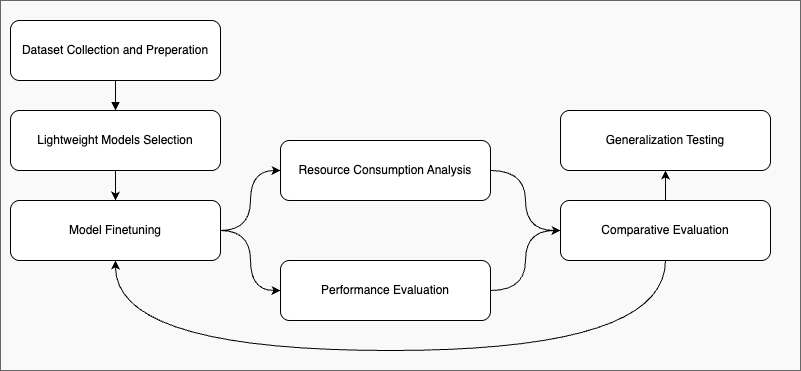
\includegraphics[width=1\linewidth]{research_methodology.drawio.png}
    \caption{Research methodology flow chart.}
    \label{fig:enter-label}
\end{figure}
\newpage
\section{Timeline}
\begin{table}[h]
    \centering
    \begin{tabular}{|p{2cm}|p{9cm}|}
        \hline
         \cellcolor[gray]{0.8}\textbf{Date range}&\cellcolor[gray]{0.8}\textbf{Work} \\[5pt]
         \hline
         02.03-11.03&Idea exploration \\
         12.03-19.03&Establishing shared Zotero library and collecting papers \\
         20.03-29.03&Writing the research proposal \\
         30.03-02.04&Eid Al-Fitr holiday \\
         03.04-06.04&Prepare and deliver presentation of research proposal \\
         07.04-13.04&Dataset collection and preparation \\
         14.04-21.04&Models selection \\
         22.04-05.05&Model fine-tuning \\
         06.05-12.05&Model evaluation \\
         13.05-19.05&Comparative analysis and model refinement \\
         20.05-26.05&Generalization testing \\
         27.05-02.06&Writing final documentation and presenting work \\
         \hline
    \end{tabular}   
    \caption{Timeline}
    \label{tab:my_label}
\end{table}
\section{Author Contributions}
\begin{itemize}
    \item \textbf{Waleed:} uploaded An-Najah University logo.
    \item \textbf{Ameed:} transformed the title page into LaTeX.
    \item \textbf{Ameed:} transformed the Introduction section into LaTeX.
    \item \textbf{Ameed:} changed the titles of the sections to match our research proposal and added the Author Contributions section.
    \item \textbf{Ameed:} transformed the methodology section into LaTeX.
    \item \textbf{Ameed:} uploaded research methodology flow chart and inserted it into the document.
    \item \textbf{Ameed:} created timeline table
    \item \textbf{Karim:} transformed the Literature Review section into LaTeX.
    \item \textbf{Karim:} transformed the References section into LaTeX.
    \item \textbf{All members:} Collaborated to revise the overall goal and objectives.
    \item \textbf{Ameed \& Karim:} organized pages flow and added \textbackslash newpage where necessary.
    \item \textbf{Waleed:} transformed Goal and Research Questions section into LaTeX and made it clear that we aim to do empirical comparisons.
\end{itemize}

%Add all relevant references as a bibliography.

\newpage
\bibliographystyle{plain}
\bibliography{reference}


\end{document}


